% Version control information:
%$HeadURL: https://practicas-spss.googlecode.com/svn/trunk/contrastes/contrastes.tex $
%$LastChangedDate: 2010-09-27 16:37:11 +0200 (lun, 27 sep 2010) $
%$LastChangedRevision: 3 $
%$LastChangedBy: asalber $
%$Id: contrastes.tex 3 2010-09-27 14:37:11Z asalber $

\chapter{Contraste de Hipótesis}

\section{Fundamentos teóricos}
\subsection{Inferencia estadística y contrastes de hipótesis}
Cualquier afirmación o conjetura que determina, parcial o totalmente, la distribución de una población se realiza mediante una \emph{Hipótesis Estadística}.

En general, nunca se sabe con absoluta certeza si una hipótesis es
cierta o falsa, ya que, para ello tendríamos que medir a todos los individuos de la población. Las decisiones se toman sobre una base de
probabilidad y los procedimientos que conducen a la aceptación o
rechazo de la hipótesis forman la parte de la Inferencia
Estadística que se denomina \emph{Contraste de Hipótesis}.

Una hipótesis se contrasta comparando sus predicciones con la
realidad que se obtiene de las muestras: si coinciden, dentro del
margen de error probabilísticamente admisible, mantendremos la
hipótesis; en caso contrario, la rechazamos y buscaremos nuevas
hipótesis capaces de explicar los datos observados.

\subsection{Tipos de contrastes de hipótesis}

Los contrastes de hipótesis se clasifican como:
\begin{itemize}
    \item \emph{Contrastes Paramétricos}.
    Que a su vez son de dos tipos según que:
    \begin{itemize}
        \item Se contraste un valor concreto o intervalo para los
        parámetros de la distribución de una variable aleatoria.
        Por ejemplo: podemos contrastar la hipótesis de que la
        media del nivel de colesterol en sangre en una población
        es de 180 mg/dl.
        \item Se comparen los parámetros de las distribuciones de
        dos o más variables. Por ejemplo: podemos contrastar la
        hipótesis de que la media del nivel de colesterol en
        sangre es más baja en las personas que ingieren por debajo
        de una cierta cantidad de grasas en su dieta.
    \end{itemize}
    \item \emph{Contrastes No Paramétricos}.
    En los que se contrastan las hipótesis que se imponen como
    punto de partida en los contrastes paramétricos, y que reciben
    el nombre de \emph{Hipótesis Estructurales}. Entre ellas, el modelo
    de distribución de los datos y la independencia de los mismos.
    Por ejemplo: en muchos de los contrastes paramétricos se exige
    como hipótesis de partida que los datos muestrales provengan
    de una población normal, pero precisamente éste sería el
    primer contraste al que habría que dar respuesta, puesto que
    si los datos no provienen de una población normal, las
    conclusiones obtenidas gracias a los contrastes paramétricos
    derivados pueden ser completamente erróneas.
\end{itemize}

\subsection{Elementos de un contraste}

\subsubsection{Hipótesis nula e hipótesis alternativa}

El primer punto en la realización de un contraste de hipótesis es
la formulación de la Hipótesis Nula y su correspondiente Hipótesis
Alternativa.

Llamaremos \emph{Hipótesis Nula} a la hipótesis que se contrasta.
Se suele representar como $H_0$ y representa la hipótesis que
mantendremos a no ser que los datos observados en la muestra
indiquen su falsedad, en términos probabilísticos.

El rechazo de la hipótesis nula lleva consigo la aceptación
implícita de la \emph{Hipótesis Alternativa}, que se suele
representar como $H_1$. Para cada $H_0$ tenemos dos $H_1$
diferentes según que el contraste sea de tipo \emph{Bilateral}, si
desconocemos la dirección en que $H_0$ puede ser falsa, o
\emph{Unilateral}, si sabemos en qué dirección $H_0$ puede ser
falsa. Y el Unilateral se clasifica como \emph{Con Cola a la
Derecha}, si en $H_1$ sólo englobamos valores mayores del
parámetro para el que planteamos el contraste que el que aparecen
en $H_0$, y \emph{Con Cola a la Izquierda}, si en $H_1$ sólo
englobamos valores menores.


En la siguiente tabla se formulan tanto $H_0$ como $H_1$ en
contrastes paramétricos, para un parámetro cualquiera, que
denominaremos $\theta$, de una población, y para la comparación de dos
parámetros, $\theta_1$ y $\theta_2$, de dos poblaciones.

\begin{center}
\begin{tabular}{|l|l|l|}
\cline{2-3}
\multicolumn{1}{l|}{} & \multicolumn{1}{c|}{$H_0$} & \multicolumn{1}{c|}{$H_1$} \\
\hline
Bilateral en una población & \multicolumn{1}{c|}{$\theta=\theta_0$} & \multicolumn{1}{c|}{$\theta\neq{\theta_0}$} \\
\hline
Unilateral en una población & \multicolumn{1}{c|}{$\theta=\theta_0$} & \multicolumn{1}{c|}{$\theta>\theta_0$ (Cola a la dcha.) ó $\theta<\theta_0$ (Cola a la Izda.)} \\
\hline
Bilateral en dos poblaciones & \multicolumn{1}{c|}{$\theta_1=\theta_2$} & \multicolumn{1}{c|}{$\theta_1\neq{\theta_2}$} \\
\hline
Unilateral en dos poblaciones & \multicolumn{1}{c|}{$\theta_1=\theta_2$} & \multicolumn{1}{c|}{$\theta_1>\theta_2$ ó $\theta_1<\theta_2$} \\
\hline
\end{tabular}
\end{center}

\begin{ejemplo}
Supongamos que, gracias a datos previos, conocemos que la media del nivel de
colesterol en sangre en una determinada población es 180 mg/dl, y suponemos que
la aplicación de una cierta terapia ha podido influir (ya sea para aumentar o
para disminuir) en dicha media. Para formular $H_0$ debemos tener en cuenta que
la hipótesis nula siempre es conservadora, es decir, no cambiaremos nuestro
modelo si no hay evidencias probabilísticamente fuertes de que ha dejado de ser
válido. Según esto, la hipótesis nula será que la media no ha cambiado:
\[
H_0: \mu = 180.
\]
Una vez fijada la hipótesis nula, para formular la hipótesis alternativa
debemos tener en cuenta que se trata de un contraste bilateral, ya que no
conocemos, a priori, el sentido de la variación de la media (si será mayor o
menor de 180 mg/dl). Por tanto, la hipótesis alternativa es que la media es
distinta de 180 mg/dl:
\[H_1: \mu \neq 180.\]

Por otro lado, si presumimos que la aplicación de la terapia ha servido para
disminuir el nivel de colesterol, estamos ante un contraste
unilateral en el que la hipótesis nula sigue siendo que la media
no ha cambiado, y la alternativa es que ha
disminuido:
\begin{align*}
H_0 &: \mu = 180,\\
H_1 &: \mu < 180.
\end{align*}
\end{ejemplo}

Normalmente, el objetivo del investigador es rechazar la hipótesis nula para
probar la certeza de la hipótesis alternativa, y esto sólo lo hará cuando haya
pruebas suficientemente significativas de la falsedad de $H_0$. Si los datos
observados en la muestra no aportan estas pruebas, entonces se mantiene la
hipótesis nula, y en este sentido se dice que es la hipótesis conservadora.
Pero conviene aclarar que aceptar la hipótesis nula no significa que sea
cierta, sino que no tenemos información suficiente o evidencia estadística
para rechazarla.

\subsubsection{Errores en un contraste. Nivel de significación y potencia}

Como ya hemos comentado, la aceptación o rechazo de $H_0$ siempre se realiza en
términos probabilísticos, a partir de la información obtenida en la muestra.
Esto supone que nunca tendremos absoluta seguridad de conocer la certeza o
falsedad de una hipótesis, de modo que al aceptarla o rechazarla es posible
que nos equivoquemos.

Los errores que se pueden cometer en un contraste de hipótesis son
de dos tipos:

\begin{itemize}
    \item \textbf{Error de tipo I}: se produce cuando rechazamos $H_0$
    siendo correcta.
    \item \textbf{Error de tipo II}: se produce cuando aceptamos $H_0$
    siendo falsa.
\end{itemize}

La probabilidad de cometer un error de tipo I se conoce como \emph{Nivel de
Significación} del contraste y se designa por \[ \alpha=P(\textrm{Rechazar
}H_0|H_0\textrm{ es cierta}).\] Y la probabilidad de cometer un error de tipo
II se designa por \[\beta=P(\textrm{Aceptar }H_0|H_0\textrm{ es falsa}).\]

Así pues, al realizar un contraste de hipótesis, pueden darse las cuatro
situaciones que aparecen esquematizadas en el cuadro~\ref{t:errores}.

\begin{table}[h!]
\centering
\begin{tabular}{|m{2.5cm}|m{3.5cm}|m{3.5cm}|}
\cline{2-3}
\multicolumn{1}{l|}{} & \multicolumn{2}{c|}{Realidad} \\
\hline
Decisión & \multicolumn{1}{c|}{$H_0$ cierta} & \multicolumn{1}{c|}{$H_0$ falsa} \\
\hline
Aceptar $H_0$ & \multicolumn{1}{m{3.5cm}|}{\centering Decisión correcta \newline (Probabilidad $1-\alpha$) } &
\multicolumn{1}{m{3.5cm}|}{\centering Error de Tipo II \newline (Probabilidad $\beta$)} \\
\hline
Rechazar $H_0$ & \multicolumn{1}{m{3.5cm}|}{\centering Error de Tipo I \newline (Probabilidad $\alpha$)} & \multicolumn{1}{m{3.5cm}|}{\centering Decisión correcta \newline (Probabilidad $1-\beta$)} \\
\hline
\end{tabular}
\caption{Tipos de errores en un contraste de hipótesis.} \label{t:errores}
\end{table}



Puesto que lo interesante en un contraste es rechazar la hipótesis nula, lo
que más interesa controlar es el riesgo de equivocación si se rechaza, es
decir el error del tipo I. Por tanto, $\alpha$ se suele fijar a niveles bajos,
ya que cuanto más pequeño sea, mayor seguridad tendremos al rechazar la
hipótesis nula. Los niveles más habituales a los que se fija $\alpha$ son
$0.1$, $0.05$ y $0.01$.

Una vez controlado el error de tipo I, también es interesante controlar el
error del tipo II. Ahora bien, el valor de $\beta$ se calcula partiendo de que
la hipótesis nula es falsa, es decir $\theta\neq \theta_0$ (o $\theta_1\neq
\theta_2$ en el caso de dos poblaciones), pero esto engloba infinitas
posibilidades, de manera que para poder calcularlo no queda más remedio que
fijar $H_1$ dando un único valor al parámetro. En este caso, se define la
\emph{Potencia del Contraste} como la probabilidad de rechazar $H_0$ cuando la
hipótesis alternativa fijada es verdadera, y vale $1-\beta$. Resulta evidente
que para un nivel de significación dado, un contraste será mejor cuanta más potencia tenga.

Como la potencia depende del valor del parámetro fijado en la hipótesis
alternativa, se puede definir una función para la potencia como
\[ \textrm{Potencia} (x)=P(\textrm{Rechazar }H_0|\theta=x),\]
que indica la probabilidad de rechazar $H_0$ para cada valor del parámetro
$\theta$. Esta función se conoce como \emph{curva de potencia}.

Por otro lado, $\beta$ también depende de $\alpha$ ya que al disminuir
$\alpha$, cada vez es más difícil rechazar $H_0$, y por tanto, la probabilidad
de aceptar la hipótesis nula siendo falsa aumenta. En consecuencia, y como
veremos más adelante, la única forma de disminuir $\beta$ y ganar potencia, una
vez fijado $\alpha$, es aumentando el tamaño de la muestra.


\subsubsection{Estadístico del contraste y regiones de aceptación y rechazo}

La decisión entre la aceptación o el rechazo de $H_0$ que se plantea en el
contraste, se realiza a partir de un estadístico en el muestreo, relacionado con
el parámetro o característica que queremos contrastar, y cuya distribución debe
ser conocida suponiendo cierta $H_0$ y una vez fijado el tamaño de la muestra.
Este estadístico recibe el nombre de \emph{Estadístico del Contraste}.

Para cada muestra el estadístico del contraste toma un valor concreto que recibe
el nombre de \emph{estimación del estadístico}. A partir de esta
estimación tomaremos la decisión de aceptar o rechazar la hipótesis nula.
Si la estimación difiere demasiado del valor que propone $H_0$ para el
parámetro, entonces rechazaremos $H_0$, mientras que si no es demasiado
diferente la aceptaremos.

La magnitud de la diferencia que estamos dispuestos a tolerar entre la
estimación y el valor del parámetro para mantener la hipótesis nula, depende de
la probabilidad de error de tipo I que estemos dispuestos a asumir. Si
$\alpha$ es grande, pequeñas diferencias pueden ser suficientes para rechazar
$H_0$, mientras que si $\alpha$ es muy pequeño, sólo rechazaremos $H_0$ cuando
la diferencia entre el estimador y el valor del parámetro según $H_0$, sea muy
grande. De esta manera, al fijar el nivel de significación $\alpha$, el
conjunto de valores que puede tomar el estadístico del contraste queda divido
en dos partes: la de las estimaciones que conducirían a la aceptación de $H_0$,
que se denomina \emph{Región de Aceptación}, y la de las estimaciones que
conducirían al rechazo de $H_0$, que se denomina \emph{Región de Rechazo}.

Si llamamos al estadístico del contraste $\hat{\theta}$, entonces, dependiendo
de si el contraste es unilateral o bilateral, tendremos las siguientes
regiones de aceptación y rechazo:
\[
\begin{array}{|c|c|c|}
\hline
\textrm{Contraste} & \textrm{Región de Aceptación} & \textrm{Región de Rechazo} \\
\hline
\begin{array}{l}
H_0:\ \theta=\theta_0\\
H_1:\ \theta\neq \theta_0
\end{array}
& \{\hat{\theta}_{1-\alpha/2}\leq \hat{\theta}\leq \hat{\theta}_{\alpha/2}\} &
\{\hat{\theta}<\hat{\theta}_{1-\alpha/2}\}\cup \{
\hat{\theta}>\hat{\theta}_{\alpha/2}\}\\
\hline
\begin{array}{l}
H_0:\ \theta=\theta_0\\
H_1:\ \theta<\theta_0
\end{array}
& \{\hat{\theta}\geq\hat{\theta}_{1-\alpha}\} &
\{\hat{\theta}<\hat{\theta}_{1-\alpha}\}\\
\hline
\begin{array}{l}
H_0:\ \theta=\theta_0\\
H_1:\ \theta>\theta_0
\end{array}
& \{\hat{\theta}\leq \hat{\theta}_{\alpha}\} &
\{\hat{\theta}>\hat{\theta}_{\alpha}\}\\
\hline
\end{array}
\]

donde $\hat{\theta}_{1-\alpha}$ y $\hat{\theta}_{\alpha}$ son valores tales
que $P(\hat{\theta}<\hat{\theta}_{1-\alpha}|\theta=\theta_0)=\alpha$ y
$P(\hat{\theta}>\hat{\theta}_{\alpha}|\theta=\theta_0)=\alpha$, tal y como se
muestra en las figuras~\ref{g:regiones_contraste_bilateral} y \ref{g:regiones_contraste_unilateral}.

\begin{figure}[h!]
\begin{center}
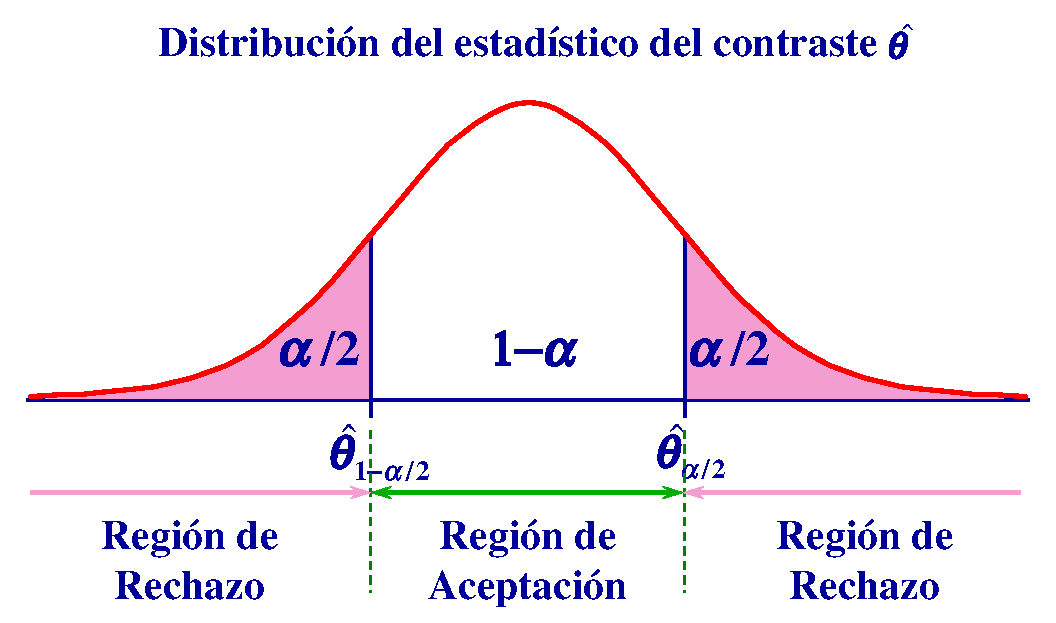
\includegraphics[scale=0.5]{contrastes/regionesbilateral}
\caption{Regiones de aceptación y rechazo en un contraste
bilateral.}\label{g:regiones_contraste_bilateral}
\end{center}
\end{figure}

\begin{figure}[h!]
\begin{center}
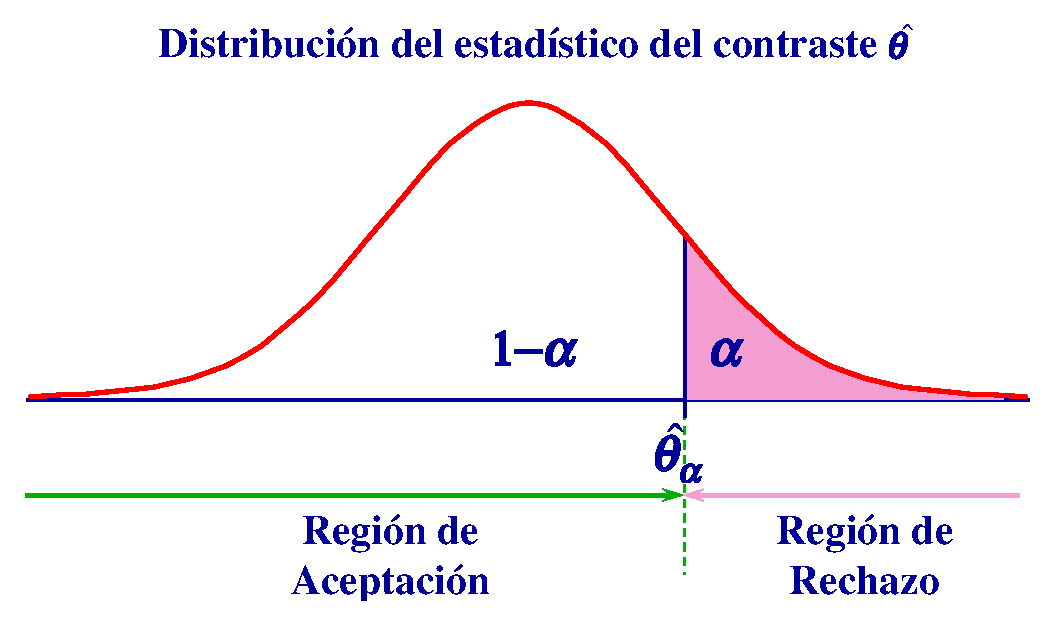
\includegraphics[scale=0.5]{contrastes/regionesunilateral}
\caption{Regiones de aceptación y rechazo en un contraste
unilateral.}\label{g:regiones_contraste_unilateral}
\end{center}
\end{figure}

En resumen, una vez que tenemos el estadístico del contraste y hemos fijado el
nivel de significación $\alpha$, las regiones de aceptación y rechazo quedan
delimitadas, y ya sólo queda tomar una muestra, calcular a partir de ella la 
estimación del estadístico delcontraste, y aceptar o rechazar la hipótesis 
nula, dependiendo de si la estimación cae en la región de aceptación o en la de rechazo 
respectivamente.



\subsubsection{El $p$-valor de un contraste}
Aunque ya disponemos de los elementos necesarios para realizar un contraste de
hipótesis que nos permita tomar una decisión respecto a aceptar o rechazar la
hipótesis nula, en la práctica, la decisión que se toma suele acompañarse del
grado de confianza que tenemos en la misma. Si por ejemplo, tenemos una región
de rechazo $\{\hat{\theta}>\hat{\theta}_\alpha\}$, siempre que la estimación
del estadístico del contraste caiga dentro de esta región rechazaremos $H_0$,
pero obviamente, si dicha estimación es mucho mayor que $\hat{\theta}_\alpha$
tendremos más confianza en el rechazo que si la estimación está cerca del
límite entre las regiones de aceptación y rechazo $\hat{\theta}_\alpha$. Por
este motivo, al realizar un contraste, también se calcula la probabilidad de
obtener una discrepancia mayor o igual que la observada entre el valor del
parámetro, suponiendo cierta $H_0$, y la estimación que se obtiene de los datos
muestrales. Esta probabilidad se conoce como  \emph{$p$-valor del contraste},
y en cierto modo, expresa la confianza que se tiene al tomar la decisión en el
contraste, ya que si $H_0$ es cierta y el $p$-valor es pequeño, es porque
bajo la hipótesis nula resulta poco probable encontrar una discrepancia como la
observada, y por tanto, tendremos bastante seguridad a la hora de rechazar
$H_0$. En general, cuanto más próximo esté $p$ a 1, mayor seguridad existe al
aceptar $H_0$, y cuanto más próximo esté a 0, mayor seguridad hay al
rechazarla.

El cálculo del $p$-valor dependerá de si el contraste es bilateral o
unilateral, y en este último caso de si es unilateral con cola a la derecha o
con cola a la izquierda. El $p$-valor que se obtiene para los diferentes tipos
de contrastes es el que aparece en la tabla siguiente:

\begin{center}
\renewcommand{\arraystretch}{1.2}
\begin{tabular}{|l|c|}
\hline
\multicolumn{1}{|c|}{Contraste} & $p$-valor \\
\hline
Bilateral & \multicolumn{1}{p{5.5cm}|}{$2P(\hat\theta>\hat\theta_0|H_0\textrm{ es cierta})$ si $\hat\theta>\hat\theta_0$ \textrm{ o}\newline $2P(\hat\theta<\hat\theta_0|H_0\textrm{ es cierta})$ si $\hat\theta<\hat\theta_0$} \\
\hline
Unilateral con cola a la derecha & $P(\hat\theta>\hat\theta _0|H_0\textrm{ es cierta})$ \\
\hline
Unilateral con cola a la izquierda & $P( \hat\theta  < \hat\theta _0|H_0\textrm{ es cierta})$ \\
\hline
\end{tabular}
\end{center}

En la figura~\ref{g:pvalor} se observa que el $p$-valor es el área de la cola
de la distribución (o colas si se trata de un contraste bilateral) definida a
partir del estadístico del contraste.

\begin{figure}[h!]
\begin{center}
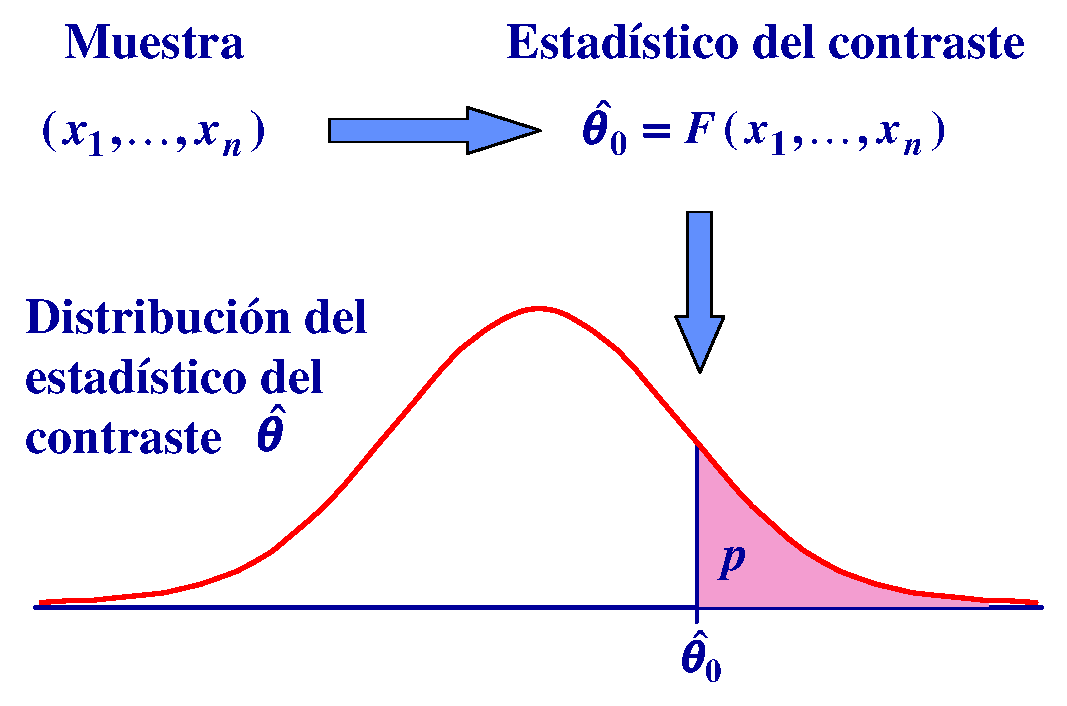
\includegraphics[scale=0.5]{contrastes/estadisticocontraste}
\caption{El $p$-valor de un contraste unilateral con cola a la derecha.}
\label{g:pvalor}
\end{center}
\end{figure}

Una vez calculado el $p$-valor, si hemos fijado el nivel de significación
$\alpha$ y han quedado delimitadas las regiones de aceptación y rechazo, el
que la estimación caiga dentro de la región de rechazo es equivalente a que
$p<\alpha$, mientras que si cae dentro de la región de aceptación, entonces
$p\geq \alpha$. Esta forma de abordar los contrastes, nos da una visión más
amplia, ya que nos da información de para qué niveles de significación puede
rechazarse la hipótesis nula, y para cuales no se puede.


\subsubsection{Contrastes y estadísticos de contraste}
Apoyándose en las distintas distribuciones en el muestreo comentadas en las
prácticas sobre intervalos de confianza, a continuación se presentan las
fórmulas para los principales estadísticos de contraste.

\subsubsection{Contraste para la media de una población normal con
varianza conocida}
\begin{itemize}
\item Hipótesis Nula: $H_0:\mu=\mu_0$
\item Estadístico del contraste:
\[
\dfrac{\bar X-\mu_0}{\sigma/\sqrt{n}}
\]
que sigue una distribución normal tipificada, $N(0,1)$.
\end{itemize}
Este contraste también es válido para la media de una población no
normal, siempre y cuando las muestras sean grandes $(n\geq 30)$,
con varianza conocida; y para la media de la diferencia de datos
emparejados, siempre y cuando la variable diferencia siga una
distribución normal con varianza conocida, o una distribución
cualquiera si la muestra es grande.

\subsubsection{Contraste para la media de una población normal con
varianza desconocida}

\begin{itemize}
\item Hipótesis Nula: $H_0:\mu=\mu_0$
\item Estadístico del contraste:
\[
\frac{\bar X-\mu_0}{\hat s/\sqrt{n}}
\]
que sigue una distribución $t$ de Student con $n-1$ grados de
libertad, $T(n-1)$.
\end{itemize}
Este contraste también es válido para la media de una población no normal en
muestras grandes $(n\geq 30)$, con varianza desconocida; y para la media de la
diferencia de datos emparejados, siempre y cuando la variable diferencia siga
una distribución normal con varianza desconocida, o una distribución
cualquiera si la muestra es grande.

\subsubsection{Contraste para la proporción en muestras grandes y
distribuciones simétricas (tanto $np$ como $n(1-p)$ deben ser
mayores que 5)}
\begin{itemize}
    \item Hipótesis Nula: $H_0: p=p_0$
    \item Estadístico del contraste:
    \[
    \frac{{\hat p - p_0 }}{{\sqrt {\frac{{\hat p\left( {1 - \hat p} \right)}}{n}} }}
    \]
    que sigue una distribución normal tipificada, $N(0,1)$.
\end{itemize}


\subsubsection{Contraste para la varianza de una población
normal}
\begin{itemize}
\item Hipótesis Nula: $H_0:\sigma^2=\sigma_0^2$
\item Estadístico del contraste:
\[
\frac{(n - 1)\hat s^2}{\sigma_0^2 }
\]
que sigue una distribución Chi-cuadrado con $n-1$ grados de libertad.
\end{itemize}

\subsubsection{Contraste para la diferencia de medias de poblaciones normales con
varianzas conocidas}
\begin{itemize}
\item Hipótesis Nula: $H_0:\mu_1=\mu_2$
\item Estadístico del contraste:
\[
\frac{\bar{X_1}-\bar{X_2}}{\sqrt{\frac{\sigma_1^2}{n_1 }+\frac{\sigma_2^2}{n_2}}}
\]
que sigue una distribución normal tipificada, $N(0,1)$.
\end{itemize}

Este contraste también es válido para la diferencia de medias de dos poblaciones no normales, siempre y cuando las muestras sean
grandes ($n_1\geq 30$ y $n_2\geq 30$), con varianzas conocidas.

\subsubsection{Contraste para la diferencia de medias de poblaciones normales con varianzas desconocidas}
\begin{itemize}
\item Hipótesis Nula: $H_0:\mu_1=\mu_2$
\item Estadístico del contraste:
\[
\frac{\bar{X_1}-\bar{X_2}}{\sqrt{\frac{\hat s_1^2}{n_1}+\frac{\hat s_2^2}{n_2}}}
\]
que sigue una distribución t de Student con $\nu$ grados de libertad, donde $\nu$ es el número entero más próximo al valor de la
expresión:
\[
\dfrac{\left( \dfrac{\hat s_1^2}{n_1}+\dfrac{\hat s_2^2}{n_2}\right)^2}{\dfrac{\left(
\dfrac{\hat s_1^2}{n_1}\right)^{2}}{n_1+1}+\dfrac{\left( \dfrac{\hat s_2^2}{n_2}\right) ^2}{n_2+1}}-2.
\]
\end{itemize}

Este contraste también es válido para la diferencia de medias de dos poblaciones no normales, siempre y cuando las muestras sean
grandes ($n_1\geq 30$ y $n_2\geq 30$), con varianzas desconocidas.

\subsubsection{Contraste para la diferencia de proporciones en muestras grandes y distribuciones simétricas ($n_1p_1$, $n_1(1-p_1)$, $n_2p_2$,
$n_2(1-p_2)$ deben ser mayores que 5)}
\begin{itemize}
\item Hipótesis Nula: $H_0:p_1=p_2$
\item Estadístico del contraste:
\[
\frac{{\hat p_1  - \hat p_2 }}{{\sqrt {\frac{{\hat p_1 \left( {1 - \hat p_1 }
\right)}}{{n_1 }} + \frac{{\hat p_2 \left( {1 - \hat p_2 } \right)}}{{n_2
}}} }}
\]
que sigue una distribución normal tipificada, $N(0,1)$.
\end{itemize}

\subsubsection{Contraste para la igualdad de varianzas de poblaciones normales}
\begin{itemize}
\item Hipótesis Nula: $H_0:\sigma_1^2=\sigma_2^2$
\item Estadístico del contraste:
\[
\frac{{\hat S^2_{1,n_1-1} }}{{\hat S^2_{2,n_2-1} }}
\]
que sigue una distribución F de Fisher con $n_1-1$ y $n_2-1$ grados de libertad.
\end{itemize}


\clearpage
\newpage


\section{Ejercicios resueltos}
\begin{enumerate}[leftmargin=*]

\item  Se analiza la concentración de principio activo en una
muestra de 10 envases tomados de un lote de un fármaco, obteniendo
los siguientes resultados en mg/mm$^{3}$:
\[
17.6-19.2-21.3-15.1-17.6-18.9-16.2-18.3-19.0-16.4
\]

Se pide:

\begin{enumerate}
\item  Crear la variable \variable{concentración}, e introducir los
datos de la muestra.

\item Realizar el contraste de hipótesis bilateral: $H_0:
\mu=18$ y $H_1:\mu\neq18$ con un nivel de significación $0.05$.
\begin{indicacion}
\begin{enumerate}
\item Seleccionar el menú \menu{Analizar\flecha Comparar medias\flecha Prueba T para una muestra}.
\item En el cuadro de diálogo que aparece, seleccionar la variable \variable{concentración} en el  campo \campo{Variables para contrastar}, introducir el valor de la media en la hipótesis nula (en este caso 18) en el campo \campo{Valor de prueba} y
hacer click en el botón \boton{Opciones}.
\item En el cuadro de diálogo que aparece, introducir el nivel de confianza del contraste en el campo \campo{Porcentaje del Intervalo
de conficanza} y hacer click sobre el botón \boton{Continuar} y \boton{Aceptar}.

Aunque el nivel de confianza no afecta al $p$-valor del contraste, que el programa denomina \resultado{sig. (bilateral)},
si afecta al intervalo de confianza que se muestra junto con el $p$-valor.
\end{enumerate}
\end{indicacion}

\item De igual manera realizar los contrastes bilaterales: $H_0:
\mu=19.5$ y $H_1:\mu\neq19.5$ con niveles de significación
$0.05$ y $0.01$. ¿Cómo afecta la disminución en el nivel de
significación en la facilidad para rechazar $H_0$?

\begin{indicacion}Seguir los mismos pasos del apartado anterior.
\end{indicacion}

\item Realizar los contrastes de hipótesis unilaterales: $H_0:
\mu=17$ y $H_1:\mu>17$, y  $H_0:\mu=17$ y $H_1:\mu<17$
con un nivel de significación de $0.1$.
\begin{indicacion}
Repetir los mismos pasos de los apartados anteriores pero teniendo en cuenta que lo que el programa denomina
\resultado{Sig.(bilateral)} es el $p$-valor del contraste bilateral; por lo tanto, para el contraste unilateral de mayor
el $p$-valor será \resultado{Sig.(bilateral)}/2, y para el contraste unilateral de menor el $p$-valor será
1-(\resultado{Sig.(bilateral)}/2).
\end{indicacion}

\item Si el fabricante del lote asegura haber aumentado la
concentración de principio activo con respecto a anteriores lotes,
en los que la media era de 17.5 mg/mm$^3$, con un nivel de
confianza del 95\%; ¿aceptamos o rechazamos lo dicho por el
fabricante?

\end{enumerate}

\item Varios investigadores desean saber si es posible concluir que dos poblaciones de niños difieren respecto a la edad promedio en la cual pueden caminar por sí solos. Los investigadores obtuvieron los siguientes datos para la edad al comenzar a andar (expresada en meses):

Muestra en la población $A$:
$9.5-10.5-9.0-9.8-10.0-13.0-10.0-13.5-10.0-9.8$

Muestra en la población $B$:
$12.5-9.5-13.5-13.8-12.0-13.8-12.5-9.5-12.0-13.5-12.0-12.0$

\begin{enumerate}

\item Crear las variables \variable{población} y \variable{edad}.

\item Realizar un contraste de hipótesis, con un nivel de
significación de $0.05$, para dar respuesta a la conclusión que
buscan los investigadores.
\begin{indicacion}
Se trata de un contraste bilateral de comparación de medias en poblaciones independientes.
\begin{enumerate}
\item Seleccionar el  menú \menu{Analizar\flecha Comparar medias\flecha Prueba T
para muestras independien\-tes}.
\item En el cuadro de diálogo que aparece, seleccionar la variable \variable{edad} en el campo \campo{Variables para contrastar}, la variable \variable{población} en el campo \campo{Variable de agrupación} y hacer click sobre el botón
\boton{Definir grupos}.
\item En el cuadro de diálogo que aparece, escribir el valor de la variable población correspondiente a la población
$A$ en el campo \campo{Grupo 1} y el correspondiente a la población $B$ en el campo \campo{Grupo 2}, y hacer click
sobre el botón \boton{Continuar} y \boton{Aceptar}.
\end{enumerate}
\end{indicacion}
\end{enumerate}


\item Algunos investigadores han observado una mayor resistencia de las vías respiratorias en fumadores que en no fumadores. Para confirmar dicha hipótesis, se realizó un estudio para comparar el porcentaje de retención traqueobronquial en las mismas personas cuando aún eran fumadoras y transcurrido un año después de dejarlo. Los resultados se indican en la tabla siguiente:

\begin{center}
\begin{tabular}{ll}
\hline
\multicolumn{2}{c}{Porcentaje de retención} \\
\hline
Cuando fumaba & Transcurrido un año sin fumar \\
\hline
\multicolumn{1}{c}{60,6} & \multicolumn{1}{c}{47,5} \\
\multicolumn{1}{c}{12,0} & \multicolumn{1}{c}{13,3} \\
\multicolumn{1}{c}{56,0} & \multicolumn{1}{c}{33,0} \\
\multicolumn{1}{c}{75,2} & \multicolumn{1}{c}{55,2} \\
\multicolumn{1}{c}{12,5} & \multicolumn{1}{c}{21,9} \\
\multicolumn{1}{c}{29,7} & \multicolumn{1}{c}{27,9} \\
\multicolumn{1}{c}{57,2} & \multicolumn{1}{c}{54,3} \\
\multicolumn{1}{c}{62,7} & \multicolumn{1}{c}{13,9} \\
\multicolumn{1}{c}{28,7} & \multicolumn{1}{c}{8,9} \\
\multicolumn{1}{c}{66,0} & \multicolumn{1}{c}{46,1} \\
\multicolumn{1}{c}{25,2} & \multicolumn{1}{c}{29,8} \\
\multicolumn{1}{c}{40,1} & \multicolumn{1}{c}{36,2} \\
\hline
\end{tabular}
\end{center}


\begin{enumerate}
\item Crear las variables \variable{antes} y \variable{después} e introducir los datos.

\item Plantear el contraste de hipótesis adecuado para confirmar o
rechazar la hipótesis de los investigadores.
\begin{indicacion}
Se trata de un contraste unilateral ($H_0: \mu_1=\mu_2$ y $H_1: \mu_1>\mu_2$) de igualdad de medias en datos pareados.
\begin{enumerate}
\item Seleccionar el menú \menu{Analizar\flecha Comparar medias\flecha Prueba T para muestras relacionadas}.
\item En el cuadro de diálogo que aparece, seleccionar ambas variables y pasarlas al campo \campo{Variables emparejadas}.
\end{enumerate}
Al tratarse de un contraste unilateral de mayor el $p$-valor será \resultado{Sig.(bilateral)}/2.
\end{indicacion}
\end{enumerate}


\item Un profesor universitario ha tenido dos grupos de clase a lo
largo del año: uno con horario de mañana y otro de tarde. En el de
mañana, sobre un total de 80 alumnos, han aprobado 55; y en el de
tarde, sobre un total de 90 alumnos, han aprobado 32.

\begin{enumerate}

\item Crear las variables: \variable{grupo}, cuyos valores serán
mañana y tarde; \variable{calificación}, cuyos valores serán 1
(aprobado) y 0 (suspenso); y \variable{frecuencia}, cuyos diferentes valores
son el número de aprobados y suspensos en cada grupo.

\item Ponderar los datos mediante la variable \variable{frecuencia}.
\begin{indicacion}
\begin{enumerate}
\item Seleccionar el menú \menu{Datos\flecha Ponderar casos}.
\item En el cuadro de diálogo resultante activar la opción \campo{Ponderar casos
mediante}, seleccionar la variable \variable{frecuencia} en el campo \campo{Variable de frecuencia} y hacer click en el
botón \boton{Aceptar}.
\end{enumerate}
\end{indicacion}

\item Realizar un contraste de hipótesis para determinar si el
factor horario ha sido o no determinante en la proporción de
suspensos con un nivel de significación $0.05$
\begin{indicacion}
Se trata de un contraste bilateral de comparación de medias en poblaciones independientes.
\begin{enumerate}
\item Seleccionar el menú \menu{Analizar\flecha Comparar 
medias\flecha Prueba T para muestras independien\-tes}.
\item Seleccionar la variable \variable{calificación} en el campo \campo{Variables para contrastar}, la variable \variable{grupo} en el campo \campo{Variable de agrupación} y hacer click en el botón \boton{Definir grupos}.
\item En el cuadro de diálogo que aparece introducir en el campo \campo{Grupo 1} el valor de la variable
\variable{grupo} correspondiente al grupo de mañana y en el campo \campo{Grupo 2} el correspondiente al grupo de tarde,
y hacer click sobre el botón \boton{Continuar}.
\end{enumerate}
\end{indicacion}


\end{enumerate}

\end{enumerate}


\section{Ejercicios propuestos}
\begin{enumerate}[leftmargin=*]
\item Un grupo de médicos intenta probar que un programa de
ejercicios moderadamente activos puede beneficiar a los pacientes
que han sufrido previamente un infarto de miocardio. Para ello
escogieron once individuos para participar en el estudio y
midieron su capacidad de trabajo, entendida como el tiempo que se
tarda en alcanzar una tasa de 160 latidos por minuto mientras se
camina con una cierta velocidad sobre una cinta de andar, al
comienzo del estudio y después de 25 semanas de ejercicio
controlado. Los resultados, expresados en minutos, fueron los
siguientes:

\begin{center}
\begin{tabular}{lll}
\hline
\multicolumn{1}{c}{Sujeto} & \multicolumn{1}{c}{Antes} & \multicolumn{1}{c}{Después} \\
\hline
\multicolumn{1}{c}{1} & \multicolumn{1}{c}{7,6} & \multicolumn{1}{c}{14,7} \\
\multicolumn{1}{c}{2} & \multicolumn{1}{c}{9,9} & \multicolumn{1}{c}{14,1} \\
\multicolumn{1}{c}{3} & \multicolumn{1}{c}{8,6} & \multicolumn{1}{c}{11,8} \\
\multicolumn{1}{c}{4} & \multicolumn{1}{c}{9,5} & \multicolumn{1}{c}{16,1} \\
\multicolumn{1}{c}{5} & \multicolumn{1}{c}{8,4} & \multicolumn{1}{c}{14,7} \\
\multicolumn{1}{c}{6} & \multicolumn{1}{c}{9,2} & \multicolumn{1}{c}{14,1} \\
\multicolumn{1}{c}{7} & \multicolumn{1}{c}{6,4} & \multicolumn{1}{c}{13,2} \\
\multicolumn{1}{c}{8} & \multicolumn{1}{c}{9,9} & \multicolumn{1}{c}{14,9} \\
\multicolumn{1}{c}{9} & \multicolumn{1}{c}{8,7} & \multicolumn{1}{c}{12,2} \\
\multicolumn{1}{c}{10} & \multicolumn{1}{c}{10,3} & \multicolumn{1}{c}{13,4} \\
\multicolumn{1}{c}{11} & \multicolumn{1}{c}{8,3} & \multicolumn{1}{c}{14,0} \\
\hline
\end{tabular}
\end{center}
¿Sostienen estos datos el argumento de los investigadores?

\item Se acepta generalmente que existen diferencias ligadas al
sexo relacionadas con la respuesta a la tensión producida por el
calor. Para comprobarlo, se sometió a un grupo de 10 hombres y 8
mujeres a un programa de ejercicios duros, en un medio con
temperatura alta (40 ºC) y sin posibilidad de beber. La variable
de interés medida fue el porcentaje de peso corporal perdido. Se
obtuvieron los datos siguientes:

\begin{center}
\begin{tabular}{ll|ll}
\hline
\multicolumn{2}{c}{Varones} & \multicolumn{2}{c}{Mujeres} \\
\hline
2,9 & 3,7 & 3,0 & 3,8 \\
3,5 & 3,8 & 2,5 & 4,1 \\
3,9 & 4,0 & 3,7 & 3,6 \\
3,8 & 3,6 & 3,3 & 4,0 \\
3,6 & 3,7 &  &  \\
\hline
\end{tabular}
\end{center}
Según los datos recogidos, ¿hay diferencias en el porcentaje medio
de peso corporal perdido como respuesta al ejercicio físico
desarrollado en alta temperatura entre hombres y mujeres?
\end {enumerate}
